\documentclass[border=8pt]{standalone}
\usepackage{mathpazo}
\usepackage{tikz}
\usetikzlibrary{arrows.meta}

\definecolor{stblue}{HTML}{7B97AD}
\definecolor{rwgold}{HTML}{B8995E}
\definecolor{sage}{HTML}{7A9A7E}
\definecolor{terracotta}{HTML}{C47A6A}
\definecolor{dkbrown}{HTML}{3D3530}
\definecolor{wmgray}{HTML}{7B7067}
\definecolor{lavender}{HTML}{907EA0}
\definecolor{goldfill}{HTML}{F5EFE4}
\definecolor{bluefill}{HTML}{E8EDF2}
\definecolor{sagefill}{HTML}{E8F0E9}
\definecolor{lavfill}{HTML}{EDE8F0}
\definecolor{terrafill}{HTML}{F2E6E3}

\begin{document}
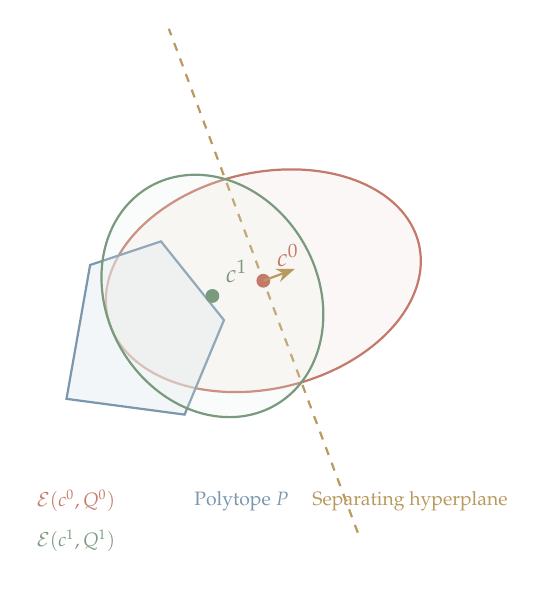
\begin{tikzpicture}[>=Stealth]

% Original ellipsoid E(c0, Q0): center (2.5, 2)
% L0 = [[2,0],[0.25,1.39194109]]
% Semi-axes: need to find rotation and radii
% Q0 = L0 L0^T = [[4, 0.5],[0.5, 2.0]]
% eigenvalues: (3+sqrt(5))/2 ~ 4.118, (3-sqrt(5))/2 ~ 1.882... wait let me recalculate
% Q = [[4, 0.5],[0.5, 0.0625+1.9375]] = [[4, 0.5],[0.5, 1.9975]]
% Actually L0 L0^T = [[4, 0.5],[0.5, 0.0625 + 1.93808...]] = [[4, 0.5],[0.5, 2.0006]]
% approximately [[4, 0.5],[0.5, 2]]
% rotation angle: atan2(2*0.5, 4-2)/(2) = atan(0.5) / 2 ~ 13.28 deg
% eigenvalues: 3 +/- sqrt(1+0.25) = 3 +/- 1.118 -> 4.118, 1.882
% semi-axes: sqrt(4.118) = 2.029, sqrt(1.882) = 1.372
% For simplicity, use the parametric form from Plotly directly:
% x(t) = 2*cos(t) + 2.5, y(t) = 0.25*cos(t) + 1.392*sin(t) + 2

% Draw original ellipsoid
\draw[terracotta, thick, fill=terrafill, fill opacity=0.3]
  plot[domain=0:360, samples=200, smooth]
  ({2*cos(\x) + 2.5}, {0.25*cos(\x) + 1.392*sin(\x) + 2});

% Polytope P
\fill[bluefill, opacity=0.5]
  (0,0.5) -- (1.5,0.3) -- (2.0,1.5) -- (1.2,2.5) -- (0.3,2.2) -- cycle;
\draw[stblue, thick]
  (0,0.5) -- (1.5,0.3) -- (2.0,1.5) -- (1.2,2.5) -- (0.3,2.2) -- cycle;

% Separating hyperplane (dashed line from (3.7,-1.2) to (1.3,5.2))
\draw[rwgold, thick, dashed] (3.7,-1.2) -- (1.3,5.2);

% New ellipsoid E(c1, Q1): center (1.853, 1.807)
% L1 = [[1.409,0],[-0.236,1.521]]
\draw[sage, thick, fill=sagefill, fill opacity=0.2]
  plot[domain=0:360, samples=200, smooth]
  ({1.409*cos(\x) + 1.853}, {-0.236*cos(\x) + 1.521*sin(\x) + 1.807});

% Centers
\fill[terracotta] (2.5, 2.0) circle (2.5pt);
\node[terracotta, font=\small, above right] at (2.55, 2.05) {$c^0$};

\fill[sage] (1.853, 1.807) circle (2.5pt);
\node[sage, font=\small, above right] at (1.9, 1.85) {$c^1$};

% Arrow showing gradient/normal direction from c0
\draw[->, rwgold, thick] (2.5, 2.0) -- (2.9, 2.15);

% Legend
\node[terracotta, font=\scriptsize, right] at (-0.5, -0.8) {$\mathcal{E}(c^0, Q^0)$};
\node[stblue, font=\scriptsize, right] at (1.5, -0.8) {Polytope $P$};
\node[rwgold, font=\scriptsize, right] at (3.0, -0.8) {Separating hyperplane};
\node[sage, font=\scriptsize, right] at (-0.5, -1.3) {$\mathcal{E}(c^1, Q^1)$};

\end{tikzpicture}
\end{document}
